\documentclass[11pt,letterpaper]{article}

\usepackage[margin=0.82in]{geometry}
\usepackage{fontspec}
\setmainfont{Times New Roman}
\setmonofont{Consolas}
\usepackage{amsmath,amssymb}
\usepackage{booktabs}
\usepackage{array}
\usepackage{graphicx}
\usepackage{float}
\usepackage{microtype}
\usepackage{setspace}
\usepackage{xcolor}
\usepackage{enumitem}
\usepackage[hidelinks]{hyperref}
\usepackage{fancyhdr}
\usepackage{caption}
\usepackage{multirow}
\graphicspath{{report/figures/}{figures/}}

\definecolor{navy}{HTML}{1B365D}
\definecolor{blue}{HTML}{2F75B5}
\definecolor{lightblue}{HTML}{EAF1F8}
\definecolor{lightgreen}{HTML}{EAF5EE}
\hypersetup{colorlinks=true,linkcolor=navy,urlcolor=navy,citecolor=navy}
\pagestyle{fancy}
\fancyhf{}
\fancyhead[L]{\small COMP 345 \textperiodcentered{} Foundations of Machine Learning}
\fancyhead[R]{\small Midterm Report \textperiodcentered{} Cuisine Classification}
\fancyfoot[C]{\small \thepage}
\setlength{\headheight}{14pt}
\setstretch{1.03}
\setlist{leftmargin=1.3em,itemsep=0.16em,topsep=0.22em}
\setlength{\parskip}{0.32em}
\setlength{\parindent}{0pt}
\setlength{\emergencystretch}{3em}
\newcommand{\tfidf}{TF-IDF}
\newcommand{\embed}{Gemini embedding}
\newcommand{\macrof}{macro-F1}
\newcommand{\workflowbox}[1]{\fcolorbox{navy}{lightblue}{\parbox[c][1.22cm][c]{0.185\linewidth}{\centering\small #1}}}
\newcommand{\repolink}{\url{https://github.com/Karmin77/COMP345ProjectCuisine}}
\newcommand{\archbox}[2]{\fcolorbox{navy}{lightblue}{\parbox[c][#1][c]{0.19\linewidth}{\centering\small #2}}}
\newcommand{\nextbox}[1]{\fcolorbox{navy}{lightgreen}{\parbox[c][1.22cm][c]{0.185\linewidth}{\centering\small #1}}}

\title{\vspace{-1.0cm}\textbf{Frozen LLM Embeddings Need Not Beat TF--IDF\\for Cuisine Classification from Ingredient Lists}\\[0.2em]\large COMP 345 Midterm Report (Checkpoint 2)}
\author{Ruoyu Gu\\COMP 345 -- Fall 2026}
\date{30 October 2026\\[0.3em]\small Code and demo notebook: \repolink}

\begin{document}
\maketitle
\thispagestyle{fancy}

\begin{abstract}
This report documents the system shown in the midterm demo: cuisine classification from ingredient lists with two finished representations, a task-specific \tfidf{} baseline and a frozen 768-dimensional \texttt{gemini-embedding-001} vector. Both share the same normalized ingredient text, the same group-aware splits, and the same PyTorch linear softmax probe, so the representation is the controlled difference. Over three outer folds at full training, \tfidf{} reaches test \macrof{} $0.7048$ and the frozen embedding $0.6462$; the paired difference is $-0.0586$ with a 95\% group-bootstrap interval of $[-0.0652,-0.0523]$. \tfidf{} leads at all eight training proportions, and the embedding loses most on small, overlapping cuisines. Yet the two models are not redundant: the embedding alone is correct on 2,025 recipes that \tfidf{} misclassifies. The proposal's two fusion methods, probability fusion and feature fusion, test exactly this complementarity; they remain part of the plan and will be reported in the final report.
\end{abstract}

\section{Problem}
The input is a recipe's ingredient list and the output is one of 20 cuisine labels. Ingredient lists are short, unordered, and highly lexical: a single ingredient such as \emph{garam masala} or \emph{fish sauce} can be decisive, while staples such as salt, garlic, and olive oil appear everywhere. The project uses this task to ask a representation question rather than to maximize accuracy:
\emph{does a frozen LLM embedding of an ingredient list classify cuisines better than classical \tfidf{} features when both are fed to the same linear probe?}
The research question and hypothesis are those of the project proposal (Version 2). The intended use is scientific analysis of representations, not a production recipe tagger.

\section{Hypothesis}
A frozen embedding probe will \emph{not} exceed the \tfidf{} probe's cuisine-classification \macrof{} by $0.02$ or more at the 100\% training setting when both use the same linear model class. We evaluate this hypothesis using the paired difference across the three outer test folds and its uncertainty interval, rather than a point estimate alone: an interval entirely below $0.02$ supports the hypothesis, an interval crossing $0.02$ is inconclusive, and an interval entirely at or above $0.02$ is evidence against it.

As in the proposal, learning curves assess whether embeddings help more in low-data settings, and we additionally test whether combining the two models' prediction probabilities (probability fusion) or their features (feature fusion) improves classification.

\section{Related approaches}
\textbf{Lexical text classification.} Bag-of-words and \tfidf{} features with a linear classifier are a long-standing, strong baseline for text classification \cite{joachims}. They keep exact, task-specific tokens, which suits ingredient lists. We use this family as the baseline.

\textbf{Frozen representations and linear probes.} A linear probe trains only a linear classifier on top of a frozen representation, so its score measures how linearly accessible the task is in that representation \cite{alainbengio}. We follow it with a hosted embedding model, \texttt{gemini-embedding-001} \cite{gemini}, used through its API as a fixed feature extractor.

\textbf{Combining representations.} Sparse lexical and dense learned features can be combined either early (concatenating features) or late (combining each model's predicted probabilities, e.g.\ by stacking \cite{stacking}). These two options are the planned feature-fusion and probability-fusion arms.

\textbf{What is different here.} Instead of maximizing leaderboard accuracy, we hold the classifier, loss, optimizer, splits, and input text fixed and change only the representation, then measure sample efficiency, per-class behaviour, and where the two representations disagree.

\section{Datasets}
We use the labelled training portion of Kaggle's What's Cooking dataset \cite{whatscooking}. The unlabeled Kaggle test file has no cuisine labels and is not used. A single record looks like this:

\begin{center}
\small
\fcolorbox{navy}{lightblue}{\parbox{0.9\linewidth}{\raggedright\ttfamily
id: 10259 \quad cuisine: greek\\
ingredients: romaine lettuce, black olives, grape tomatoes, garlic, pepper, purple onion, seasoning, garbanzo beans, feta cheese crumbles}}
\end{center}

Each ingredient is lowercased, trimmed, and whitespace-normalized; the strings are sorted and joined with newlines. This single serialization is both the \tfidf{} document and the Gemini input. Identical normalized lists form a group and never cross a split boundary, which prevents duplicate recipes from leaking between training and test. Fourteen groups (30 recipes) carry conflicting labels; they are retained and reported.

\begin{table}[H]
\centering
\caption{Dataset and frozen evaluation setup.}
\label{tab:data}
\small
\begin{tabular}{@{}lr@{}}
\toprule
Quantity & Value \\
\midrule
Labelled recipes & 39,774 \\
Normalized ingredient groups & 39,242 \\
Ambiguous groups / recipes & 14 / 30 \\
Cuisine classes & 20 \\
Outer evaluation & 3 stratified, group-aware folds \\
Validation fraction & 15\% of each development pool \\
Training proportions & 2, 5, 10, 20, 40, 60, 80, 100\% \\
Random seed & 345 \\
\bottomrule
\end{tabular}
\end{table}

\begin{table}[H]
\centering
\caption{Recipes per split in each outer fold. Every labelled recipe is a test recipe in exactly one fold.}
\label{tab:folds}
\small
\begin{tabular}{@{}lrrr@{}}
\toprule
Fold & Training pool & Validation & Test \\
\midrule
0 & 22,703 & 3,801 & 13,270 \\
1 & 22,731 & 3,798 & 13,245 \\
2 & 22,714 & 3,801 & 13,259 \\
\bottomrule
\end{tabular}
\end{table}

\section{Models / Workflow}
Figure~\ref{fig:workflow} shows the input-to-output path and Figure~\ref{fig:arch} the model architecture. The blue boxes are finished and shown in the demo; the green box is the next stage and reuses the same splits.

\begin{figure}[H]
\centering
\begin{tabular}{c@{\quad}c@{\quad}c@{\quad}c@{\quad}c}
\workflowbox{Recipe JSON\\ingredient list} & $\rightarrow$ &
\workflowbox{Normalize, sort,\\group duplicates} & $\rightarrow$ &
\workflowbox{TF-IDF branch\\or cached Gemini} \\
&& && $\downarrow$ \\
\workflowbox{Learning curve,\\per-class F1, errors} & $\leftarrow$ &
\workflowbox{3 outer folds\\$\times$ 8 proportions} & $\leftarrow$ &
\workflowbox{Shared PyTorch\\linear probe} \\
&& && $\downarrow$ \\
&& && \nextbox{Next: probability\\and feature fusion}
\end{tabular}
\caption{Workflow of the current system. The Gemini API is called only once, to build the embedding cache; every later stage runs locally from saved files.}
\label{fig:workflow}
\end{figure}

\begin{figure}[H]
\centering
\small
\begin{tabular}{@{}c@{\;}c@{\;}c@{\;}c@{\;}c@{\;}c@{\;}c@{}}
\archbox{1.22cm}{Sorted ingredient\\text $x$} & $\rightarrow$ &
\archbox{2.6cm}{\textbf{\tfidf{}} (sparse)\\$z\in\mathbb{R}^{|V|}$\\[0.35em]\emph{or}\\[0.35em]\textbf{Gemini} (frozen)\\$z\in\mathbb{R}^{768}$} & $\rightarrow$ &
\archbox{1.22cm}{Linear layer\\$Wz+b$\\$W\in\mathbb{R}^{20\times d}$} & $\rightarrow$ &
\archbox{1.22cm}{Softmax over\\20 cuisines}
\end{tabular}
\caption{Model architecture. Each run uses one representation $z$ (dimension $d$); only $W$ and $b$ are trained. $|V|$ is the \tfidf{} vocabulary fit on the current training subset.}
\label{fig:arch}
\end{figure}

\subsection{Baseline: \tfidf{}}
The vocabulary and inverse-document-frequency weights are fit on each training subset only. Validation chooses among word unigrams, word unigrams plus bigrams, and whole-ingredient tokens. Across the 24 fold-by-proportion fits, validation chose unigrams plus bigrams 14 times and unigrams 10 times; whole-ingredient tokens were never selected.

\subsection{Foundation-model integration: frozen Gemini embedding}
Each serialized recipe is sent once to Google's \texttt{gemini-embedding-001} with task type \texttt{CLASSIFICATION} and 768 output dimensions \cite{gemini}. The model is not fine-tuned; it is a frozen feature extractor. Generation is a separate, resumable command that writes a local cache. The cache used here has shape $39{,}774 \times 768$ (\texttt{float32}), contains only finite values, and is checked against the recipe-id order and a metadata fingerprint before any evaluation reads it. No labels or classifier weights are sent to the API.

\subsection{Shared linear probe}
For a representation $z(x)\in\mathbb{R}^d$, the probe is
\[
f_\theta(z)=\operatorname{softmax}(Wz+b), \qquad W\in\mathbb{R}^{20\times d},\; b\in\mathbb{R}^{20},
\]
trained with multiclass cross-entropy and Adam in PyTorch \cite{pytorch}. Learning rate and L2 weight decay are selected on validation \macrof{}; training uses batch size 512 and early stopping with patience 8. At full training the selected settings were the same for both representations in every fold (learning rate $10^{-2}$, weight decay $10^{-5}$). Because the classifier family, loss, optimizer, and selection rule are shared, differences in test scores reflect the input representation.

\section{Experiments to test the hypothesis}
The proposal's design has four methods (\tfidf{}, frozen embedding, probability fusion, feature fusion), each evaluated on the same three outer folds and eight nested training proportions, for 96 evaluation settings. This midterm checkpoint reports the two standalone methods, which give 48 fold-level test scores; the two fusion methods use the same folds and proportions and will be reported in the final report. Test folds are never used for fitting or selection; the validation slice is used only for model and hyperparameter choice.

The primary metric is test \macrof{}, which weights the 20 cuisines equally so that small classes are not hidden by Italian and Mexican. Accuracy is reported as a secondary metric. The primary test is the paired difference in \macrof{} between embedding and \tfidf{} at 100\% training. A group bootstrap with 2,000 replicates resamples whole normalized ingredient groups inside each fold, which preserves the pairing between the two methods' predictions on the same recipes.

\section{Results}
\subsection{Full-training comparison}

\begin{table}[H]
\centering
\caption{Test results at 100\% training, three outer folds.}
\label{tab:main}
\small
\begin{tabular}{@{}lcccc@{}}
\toprule
Method & Mean \macrof{} & Fold SD & Fold \macrof{} scores & Mean accuracy \\
\midrule
\tfidf{} & \textbf{0.7048} & 0.0053 & 0.6987, 0.7080, 0.7076 & \textbf{0.7820} \\
Frozen \embed{} & 0.6462 & 0.0135 & 0.6397, 0.6372, 0.6617 & 0.7631 \\
\bottomrule
\end{tabular}
\end{table}

The paired difference, embedding minus \tfidf{}, is
\[
\Delta=-0.0586, \qquad 95\%\text{ group-bootstrap interval }[-0.0652,\,-0.0523].
\]
The whole interval lies below zero and far below the $+0.02$ threshold, so the hypothesis is supported: the frozen embedding does not replace the lexical baseline on this task. The accuracy gap (1.9 points) is smaller than the \macrof{} gap (5.9 points), which already suggests that the embedding's losses are concentrated in smaller classes.

\subsection{Learning curve}

\begin{figure}[H]
\centering
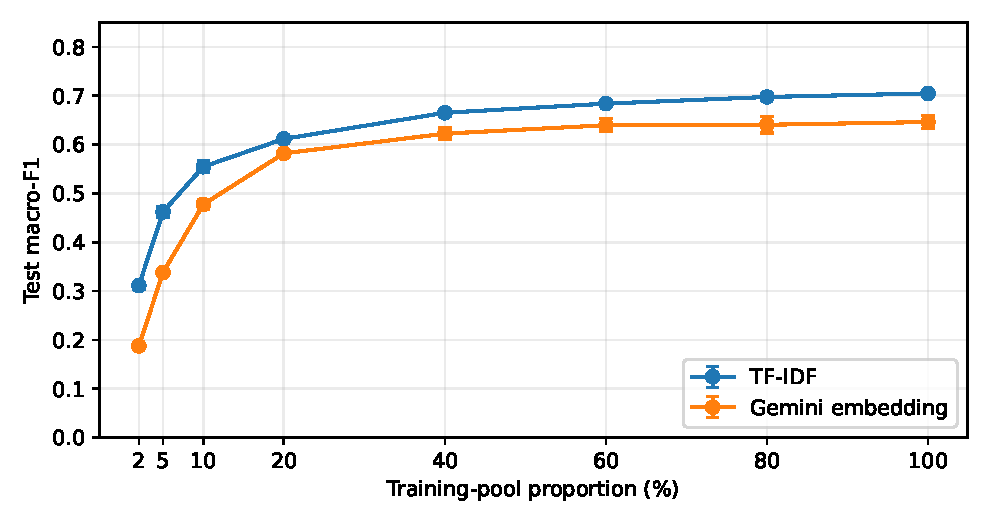
\includegraphics[width=0.78\linewidth]{midterm_learning_curve.pdf}
\caption{Test \macrof{} against training-pool proportion. Points are means over three outer folds; bars are fold standard deviations.}
\label{fig:curve}
\end{figure}

\begin{table}[H]
\centering
\caption{Learning-curve means (test \macrof{}).}
\label{tab:curve}
\small
\begin{tabular}{@{}rccc@{}}
\toprule
Training pool & \tfidf{} & Frozen embedding & Gap \\
\midrule
2\% & 0.311 & 0.188 & $-0.123$ \\
5\% & 0.462 & 0.338 & $-0.124$ \\
10\% & 0.555 & 0.478 & $-0.077$ \\
20\% & 0.612 & 0.582 & $-0.030$ \\
40\% & 0.665 & 0.622 & $-0.043$ \\
60\% & 0.684 & 0.640 & $-0.044$ \\
80\% & 0.697 & 0.641 & $-0.056$ \\
100\% & 0.705 & 0.646 & $-0.059$ \\
\bottomrule
\end{tabular}
\end{table}

\tfidf{} is ahead at every proportion. The answer to the low-data question is therefore negative in this configuration: the pretrained representation does not make the probe more sample-efficient. The gap is widest at 2--5\% training, where the smallest cuisines have only a handful to a few dozen training recipes and a 768-dimensional dense probe has too little data to separate them. The embedding curve also flattens after 60\%, while \tfidf{} keeps improving slowly.

\subsection{Per-class F1}

\begin{table}[H]
\centering
\caption{Mean per-class test F1 at 100\% training. Gap is embedding minus \tfidf{}; gaps below $-0.10$ are in bold.}
\label{tab:perclass}
\small
\begin{tabular}{@{}lccc@{\qquad}lccc@{}}
\toprule
Cuisine & \tfidf{} & Gemini & Gap & Cuisine & \tfidf{} & Gemini & Gap \\
\midrule
Brazilian & 0.612 & 0.393 & $\mathbf{-0.219}$ & Jamaican & 0.768 & 0.655 & $\mathbf{-0.113}$ \\
British & 0.460 & 0.346 & $\mathbf{-0.114}$ & Japanese & 0.744 & 0.735 & $-0.009$ \\
Cajun Creole & 0.725 & 0.721 & $-0.004$ & Korean & 0.790 & 0.719 & $-0.071$ \\
Chinese & 0.817 & 0.808 & $-0.009$ & Mexican & 0.910 & 0.909 & $-0.001$ \\
Filipino & 0.653 & 0.585 & $-0.069$ & Moroccan & 0.795 & 0.759 & $-0.036$ \\
French & 0.615 & 0.586 & $-0.029$ & Russian & 0.489 & 0.382 & $\mathbf{-0.107}$ \\
Greek & 0.750 & 0.713 & $-0.037$ & Southern US & 0.745 & 0.720 & $-0.025$ \\
Indian & 0.883 & 0.878 & $-0.005$ & Spanish & 0.536 & 0.456 & $-0.080$ \\
Irish & 0.548 & 0.427 & $\mathbf{-0.121}$ & Thai & 0.779 & 0.750 & $-0.029$ \\
Italian & 0.843 & 0.834 & $-0.010$ & Vietnamese & 0.632 & 0.548 & $-0.084$ \\
\bottomrule
\end{tabular}
\end{table}

Large, distinctive cuisines (Mexican, Indian, Italian, Chinese) are nearly tied. The embedding loses most on Brazilian, Irish, British, Jamaican, and Russian: small classes whose identity often rests on one or two rare ingredients that a dense 768-dimensional summary can blur, and which give the probe few examples to learn from.

\section{Failure analysis}
\subsection{Most frequent confusions}
Each labelled recipe is a test recipe in exactly one outer fold, so the counts below cover all 39,774 recipes using the saved 100\% predictions.

\begin{table}[H]
\centering
\caption{Five largest off-diagonal confusions (true $\rightarrow$ predicted) at 100\% training.}
\label{tab:confusions}
\small
\begin{tabular}{@{}lr@{\qquad}lr@{}}
\toprule
\multicolumn{2}{c}{\tfidf{}} & \multicolumn{2}{c}{Frozen \embed{}} \\
\midrule
French $\rightarrow$ Italian & 523 & French $\rightarrow$ Italian & 657 \\
Italian $\rightarrow$ French & 339 & Greek $\rightarrow$ Italian & 287 \\
Cajun Creole $\rightarrow$ Southern US & 260 & Spanish $\rightarrow$ Italian & 279 \\
Southern US $\rightarrow$ Italian & 205 & Cajun Creole $\rightarrow$ Southern US & 276 \\
Greek $\rightarrow$ Italian & 199 & Italian $\rightarrow$ French & 273 \\
\bottomrule
\end{tabular}
\end{table}

Both models confuse neighbouring cuisines that share ingredients and techniques. The embedding is more strongly pulled toward Italian, the largest Mediterranean class: French, Greek, and Spanish recipes all flow into it more often than under \tfidf{}.

\subsection{Where the two models disagree}

\begin{table}[H]
\centering
\caption{Agreement between the two models on all 39,774 test predictions at 100\% training.}
\label{tab:agreement}
\small
\begin{tabular}{@{}lrr@{}}
\toprule
Outcome & Recipes & Share \\
\midrule
Both correct & 28,326 & 71.2\% \\
\tfidf{} correct only & 2,779 & 7.0\% \\
\embed{} correct only & 2,025 & 5.1\% \\
Both wrong & 6,644 & 16.7\% \\
\bottomrule
\end{tabular}
\end{table}

The embedding is weaker overall, but it is not a subset of \tfidf{}: it alone gets 2,025 recipes right. If an oracle could always pick the correct model, accuracy would rise from 78.2\% to 83.3\%. That ceiling is not achievable, but it shows that there is complementary signal for fusion to look for. Three cases from the demo illustrate the categories:

\begin{itemize}
  \item \textbf{\tfidf{} only} (id 22884, British; embedding predicts Indian): \emph{white vinegar, pearl onions, cucumber, ground ginger, flour, ground turmeric, cauliflower, sugar, mustard powder}. This is a piccalilli-style pickle. Turmeric and ginger pull the dense vector toward Indian, while \tfidf{} keys on the vinegar/mustard/pearl-onion combination seen in British training recipes.
  \item \textbf{Embedding only} (id 2145, Vietnamese; \tfidf{} predicts Thai): \emph{rice vinegar, lime juice, asian fish sauce, hot chili, sugar, garlic cloves}. This is a dipping sauce (nuoc cham). Every token is common in Thai recipes, so lexical weights favour the larger class; the embedding of the whole list lands closer to Vietnamese.
  \item \textbf{Both wrong} (id 8, French; both predict Italian): \emph{whole milk, sea salt, vanilla sugar, lemon, hazelnuts, baking powder, flour, eggs, extra-virgin olive oil}. A hazelnut and olive-oil cake has no ingredient that marks it as French. No representation of this list can recover a label that the list does not contain.
\end{itemize}

The 6,644 shared errors put a practical ceiling on this task: much of the remaining error comes from overlapping cuisines and from the label itself, not from the choice of representation.

\section{Discussion and limitations}
Ingredient lists behave close to a bag-of-words problem, so exact lexical evidence is strong, and \tfidf{} with bigrams captures informative pairs directly. Compressing a whole list into 768 dense coordinates keeps general culinary similarity but can blur rare, decisive ingredients, which is exactly where the embedding loses (small classes, Mediterranean neighbours). This is a result about one embedding model, one serialization, one probe family, and one dataset, not a claim that foundation-model embeddings are generally worse.

Limitations of this checkpoint: one embedding model and one fixed serialization; one split seed; a linear probe only. Outer-fold training pools overlap, so fold standard deviations are descriptive rather than estimates over independent datasets, and the bootstrap is conditional on the fitted predictions. The 30 ambiguous recipes and the cuisine overlap mean that perfect accuracy is not attainable. Fusion results are not part of this checkpoint, so this report makes no claim about complementarity beyond the disagreement counts in Table~\ref{tab:agreement}.

\section{Status and plan for the final stretch}
\textbf{Done and shown in the midterm demo.} Shared normalization and duplicate grouping; frozen group-aware splits; the \tfidf{} baseline; the validated 39,774-recipe Gemini cache; the shared PyTorch probe; the eight-point learning curve; the paired bootstrap comparison; per-class F1, confusions, and agreement analysis. The demo notebook (\texttt{demo/COMP345\_midterm\_demo.ipynb}) reads only saved files: it makes no Gemini call and trains nothing. Source code, the split manifest, the midterm results tables, and this report are in the GitHub repository (\repolink). The Kaggle data and the large embedding and prediction archives are not committed; the README explains how to download or regenerate them.

\textbf{Next, toward the 2 December deliverables.}
\begin{itemize}
  \item \textbf{Probability fusion:} combine the two probes' class probabilities with weights learned from group-aware out-of-fold predictions, so no test information enters the combiner.
  \item \textbf{Feature fusion:} concatenate the \tfidf{} and embedding features and train the same linear probe, then compare it with both standalone arms on the same folds and proportions.
  \item \textbf{Fusion failure analysis:} count rescue cases (fusion fixes a standalone error) and regressions (fusion breaks a standalone success), and check whether fusion helps the small classes in Table~\ref{tab:perclass}.
  \item \textbf{Codebase and presentation:} keep the fresh-clone run in the README working, and prepare the 10-page report, poster, and live demo around the complete experiment.
\end{itemize}

\begin{thebibliography}{9}
\bibitem{joachims}
T. Joachims, ``Text Categorization with Support Vector Machines: Learning with Many Relevant Features,'' in \emph{ECML}, 1998.

\bibitem{alainbengio}
G. Alain and Y. Bengio, ``Understanding Intermediate Layers Using Linear Classifier Probes,'' arXiv:1610.01644, 2016.

\bibitem{stacking}
D. H. Wolpert, ``Stacked Generalization,'' \emph{Neural Networks}, 5(2), 241--259, 1992.

\bibitem{whatscooking}
Kaggle, ``What's Cooking?'' Dataset, \url{https://www.kaggle.com/c/whats-cooking}.

\bibitem{gemini}
Google, ``Gemini API embeddings,'' \url{https://ai.google.dev/gemini-api/docs/embeddings}.

\bibitem{pytorch}
A. Paszke et al., ``PyTorch: An Imperative Style, High-Performance Deep Learning Library,'' in \emph{NeurIPS}, 2019.
\end{thebibliography}

\end{document}
